\documentclass[11pt,letterpaper]{article}
\usepackage[top=0.85in,bottom=0.85in,left=1in,right=1in]{geometry}
\usepackage{amsmath,amssymb}
\usepackage{xcolor}
\usepackage{mdframed}
\usepackage{graphicx}
\usepackage{fancyhdr}
\usepackage{booktabs}
\usepackage{cancel}

\graphicspath{{cs_crops/}{./}}

\definecolor{teal}{HTML}{0F6E56}\definecolor{tealbg}{HTML}{E1F5EE}
\definecolor{coral}{HTML}{993C1D}\definecolor{coralbg}{HTML}{FAECE7}
\definecolor{purple}{HTML}{534AB7}\definecolor{purplebg}{HTML}{EEEDFE}
\definecolor{amber}{HTML}{854F0B}\definecolor{amberbg}{HTML}{FAEEDA}

\newmdenv[linewidth=1pt,linecolor=teal,backgroundcolor=tealbg!30,
  innerleftmargin=6pt,innerrightmargin=6pt,
  innertopmargin=4pt,innerbottommargin=4pt,
  skipabove=4pt,skipbelow=6pt]{cssnip}

\newmdenv[linewidth=1pt,linecolor=coral,backgroundcolor=coralbg!30,
  innerleftmargin=6pt,innerrightmargin=6pt,
  innertopmargin=4pt,innerbottommargin=4pt,
  skipabove=4pt,skipbelow=4pt]{notebox}

\pagestyle{fancy}\fancyhf{}
\renewcommand{\headrulewidth}{0.4pt}
\fancyhead[L]{\textbf{ECE332 Spring 2026 --- HW2 Generated Answers}}
\fancyhead[R]{Bao Nguyen}
\fancyfoot[C]{\thepage}

\setlength{\parindent}{0pt}\setlength{\parskip}{4pt}

\newcommand{\probhead}[2]{%
  \colorbox{purplebg}{\parbox{\dimexpr\linewidth-2\fboxsep}%
  {\color{purple}\large\textbf{Problem #1 \hfill #2}}}}

\begin{document}

\begin{center}
{\Large\textbf{ECE 332 --- Homework 2: Generated Answers from Cheat Sheet}}\\[4pt]
{\small Each solution shows the cheat sheet snippet used, then the answer.}
\end{center}

\vspace{6pt}

%======================================================
\probhead{1 --- Plane Wave $E$ and $H$ with Phase Constant}{10 pts}

\textbf{Setup:} 1 GHz wave traveling $+\hat{y}$ in lossless nonmagnetic medium with $\varepsilon_r=9$. $\mathbf{E}$ along $\hat{x}$, peak 6 V/m, $|E|=4$ V/m at $t=0$, $y=2$ cm.

\begin{cssnip}

\includegraphics[width=0.49\linewidth]{cs_waveparams}\hfill

\includegraphics[width=0.49\linewidth]{cs_losslessEH}
\end{cssnip}

\textbf{Parameters from the cheat sheet order $\omega\!\to\!u_p\!\to\!k\!\to\!\lambda\!\to\!\eta$:}
\[\omega = 2\pi f = 2\pi\times10^9~\text{rad/s},\qquad
  k = \tfrac{\omega\sqrt{\varepsilon_r}}{c} = \tfrac{2\pi\times10^9\sqrt{9}}{3\times10^8} = 20\pi~\text{rad/m}\]

\textbf{General $\mathbf{E}$ form} (wave in $+\hat{y}$ so argument is $\omega t - ky$):
\[\mathbf{E}(y,t) = 6\cos(\omega t - ky + \phi_0)\,\hat{x}~\text{V/m}\]

\textbf{Find $\phi_0$ from the given condition} $|E|=4$ at $t=0$, $y=0.02$ m:
\[4 = 6\cos(-0.4\pi + \phi_0)\;\Rightarrow\;-0.4\pi+\phi_0 = \cos^{-1}(2/3) = 0.84~\text{rad}\]
\[\boxed{\phi_0 = 2.1~\text{rad}}\]

\[\boxed{\mathbf{E}(y,t) = 6\cos\!\big((2\pi\times10^9)t - (20\pi)y + 2.1\big)\,\hat{x}~\text{V/m}}\]

\textbf{Magnetic field via $\mathbf{H} = \frac{1}{\eta}(\hat{k}\times\mathbf{E})$:}
\[\eta = \tfrac{\eta_0}{\sqrt{\varepsilon_r}} = \tfrac{377}{3} \approx 125.7~\Omega,\qquad
  \hat{y}\times\hat{x} = -\hat{z}\]
\[\boxed{\mathbf{H}(y,t) = -\tfrac{6}{125.7}\cos\!\big((2\pi\times10^9)t - (20\pi)y + 2.1\big)\,\hat{z}~\text{A/m}}\]

\newpage
%======================================================
\probhead{2 --- $f, u_p, \lambda, k, \eta$ and $\mathbf{H}$}{12 pts}

\textbf{Setup:} $\mathbf{E} = 20\cos((6\pi\!\times\!10^9)t - kz)\,\hat{y}$ V/m, lossless nonmagnetic, $\varepsilon_r=2.56$.

\begin{cssnip}

\includegraphics[width=0.49\linewidth]{cs_waveparams}\hfill

\includegraphics[width=0.49\linewidth]{cs_kxE}
\end{cssnip}

\textbf{(a)} Apply the parameter chain in order:
\begin{align*}
f &= \omega/(2\pi) = 3\times10^9~\text{Hz}\\
u_p &= c/\sqrt{\varepsilon_r} = 3\!\times\!10^8/\sqrt{2.56} = 1.875\!\times\!10^8~\text{m/s}\\
\lambda &= u_p/f = 6.25~\text{cm}\\
k &= 2\pi/\lambda = 32\pi \approx 100.5~\text{rad/m}\\
\eta &= \eta_0/\sqrt{\varepsilon_r} = 377/\sqrt{2.56} = 235.6~\Omega
\end{align*}

\textbf{(b) $\mathbf{H}$ direction from the $\hat{k}\times\hat{E}$ table:}\\
Wave in $+\hat{z}$, $\mathbf{E}$ along $\hat{y}$, so $\hat{z}\times\hat{y} = -\hat{x}$.
\[\boxed{\mathbf{H}(z,t) = -\tfrac{20}{235.6}\cos\!\big((6\pi\!\times\!10^9)t - (32\pi)z\big)\,\hat{x} = -0.0849\cos(\cdot)\,\hat{x}~\text{A/m}}\]

\newpage
%======================================================
\probhead{3 --- Polarization Analysis (4 cases)}{16 pts}

\textbf{Setup:} $\mathbf{E}(z,t) = a_x\cos(\omega t - kz)\hat{x} + a_y\cos(\omega t - kz + \delta)\hat{y}$.

\begin{cssnip}
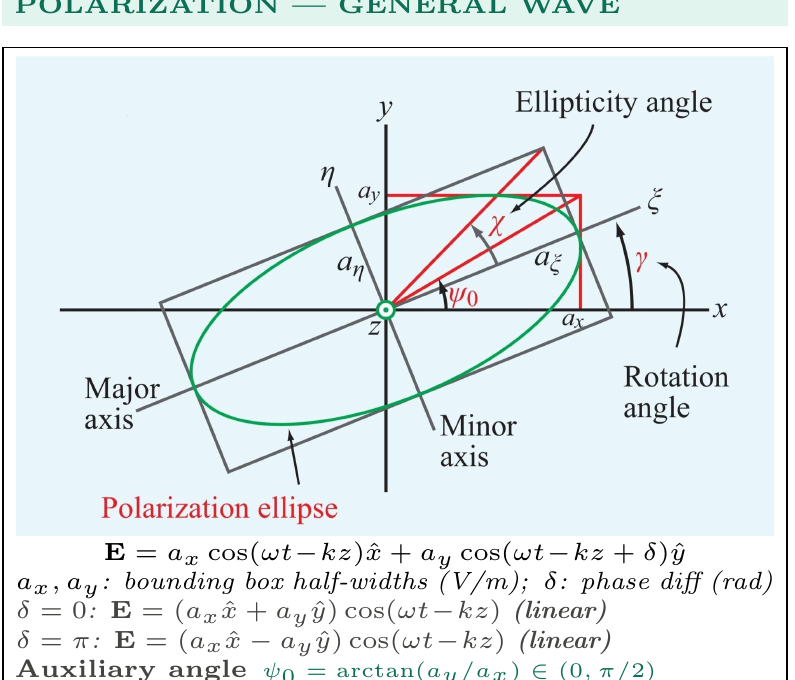
\includegraphics[width=0.49\linewidth]{cs_polarization}\hfill
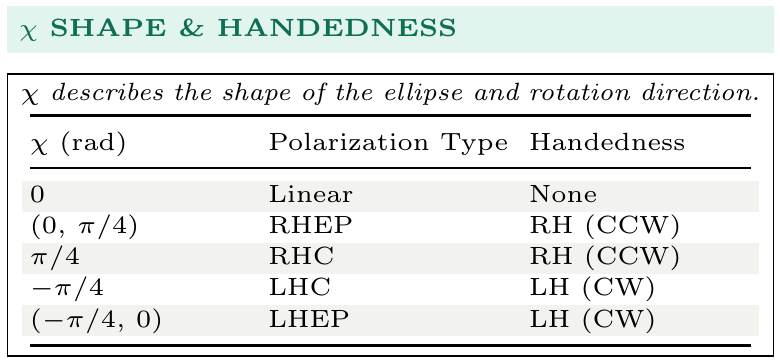
\includegraphics[width=0.49\linewidth]{cs_chi}\\[4pt]
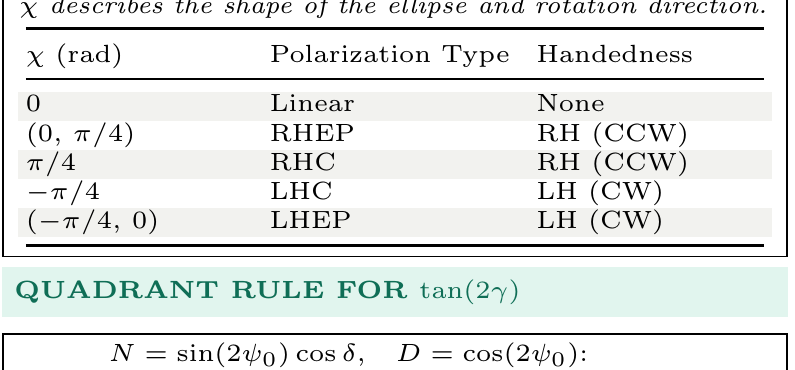
\includegraphics[width=0.49\linewidth]{cs_quadrant}\hfill
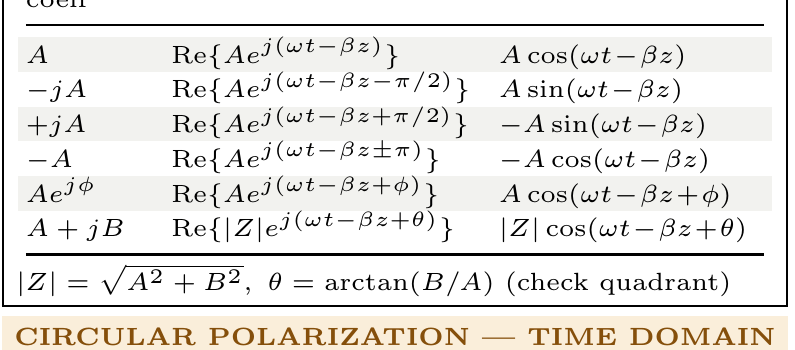
\includegraphics[width=0.49\linewidth]{cs_circular}
\end{cssnip}

\textbf{(a) $a_x=3$, $a_y=4$, $\delta=0$:} $\delta=0\Rightarrow$ linear. $R=\infty$, $\chi=0$. Rotation angle = inclination:
\[\psi = \tan^{-1}(4/3) = 0.9273~\text{rad} = 53.13^\circ \Rightarrow \boxed{\gamma=53.13^\circ,\;\chi=0}\]
\begin{center}
\includegraphics[width=0.55\linewidth]{HW2_P3a}\end{center}

\textbf{(b) $a_x=3$, $a_y=4$, $\delta=\pi$:} $\delta=\pi\Rightarrow$ linear again ($\cos(\theta+\pi)=-\cos\theta$, so $\mathbf{E}=(3\hat{x}-4\hat{y})\cos(\omega t-kz)$). $\chi=0$.
\[\psi = \tan^{-1}(-4/3) = -0.9273~\text{rad} = -53.13^\circ \Rightarrow \boxed{\gamma=-53.13^\circ,\;\chi=0}\]
\begin{center}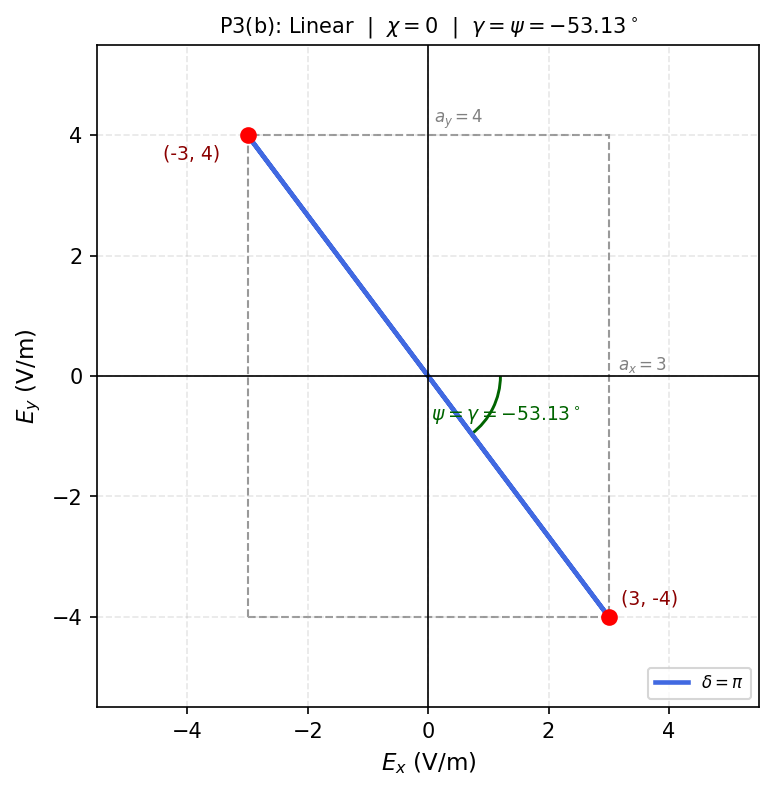
\includegraphics[width=0.55\linewidth]{HW2_P3b}\end{center}

\newpage
\textbf{(c) $a_x=3$, $a_y=3$, $\delta=\pi/4$:} elliptical. Auxiliary $\psi_0 = \tan^{-1}(1) = \pi/4$.
\[\tan 2\gamma = \tan(\pi/2)\cos(\pi/4) = \infty\sqrt{2}/2 \Rightarrow 2\gamma=\pi/2\]
\[\sin 2\chi = \sin(\pi/2)\sin(\pi/4) = \sqrt{2}/2 \Rightarrow 2\chi=\pi/4\]
\[\boxed{\gamma = \pi/4 = 45^\circ,\quad \chi = \pi/8 = 22.5^\circ}\]
$\chi>0\Rightarrow$ right-hand elliptical (RHEP).
\begin{center}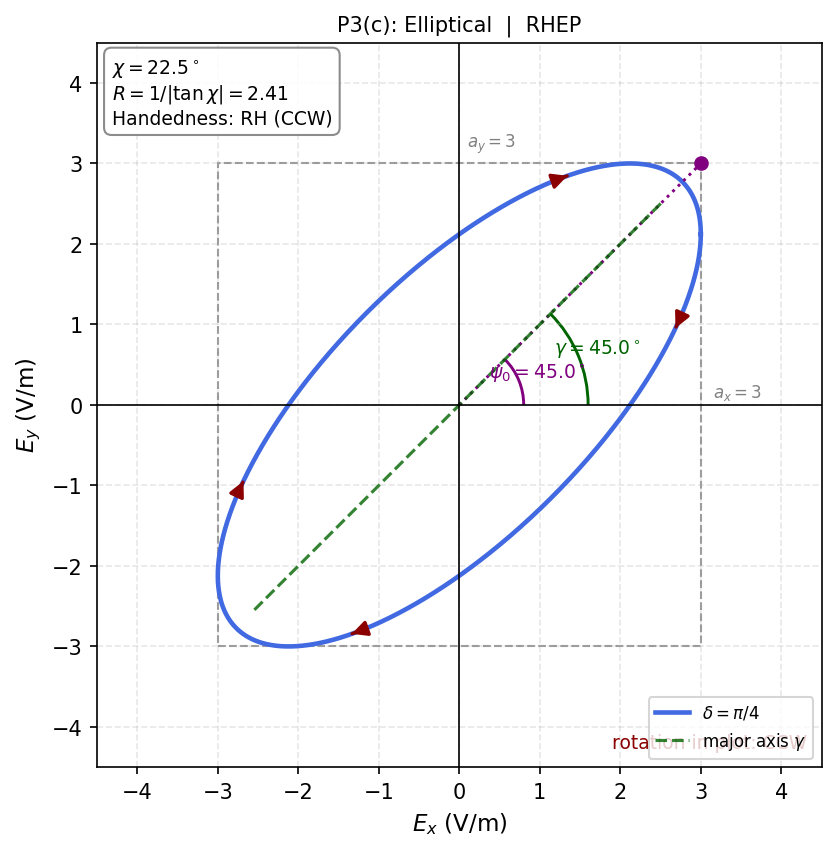
\includegraphics[width=0.55\linewidth]{HW2_P3c}\end{center}

\textbf{(d) $a_x=3$, $a_y=4$, $\delta=-3\pi/4$:} elliptical. $\psi_0=\tan^{-1}(4/3)\approx0.9273$, $2\psi_0\approx1.8546$ ($106.26^\circ$).
\[\cos\delta = -\sqrt{2}/2,\quad \sin\delta = -\sqrt{2}/2\]
\[\tan 2\gamma = \tan(1.8546)\cdot(-\sqrt{2}/2) \approx 2.4244\]
$N = \sin(2\psi_0)\cos\delta < 0$, $D = \cos(2\psi_0) < 0$ (quadrant rule: both negative)
\[2\gamma \approx -1.1796~\text{rad} = -73.73^\circ \Rightarrow \boxed{\gamma \approx -21.4^\circ}\]
\[\sin 2\chi = \sin(1.8546)\cdot(-\sqrt{2}/2) = -0.7462 \Rightarrow 2\chi \approx -0.7462~\text{rad}\Rightarrow \boxed{\chi \approx -36.9^\circ}\]
$\chi<0\Rightarrow$ left-hand elliptical (LHEP).
\begin{center}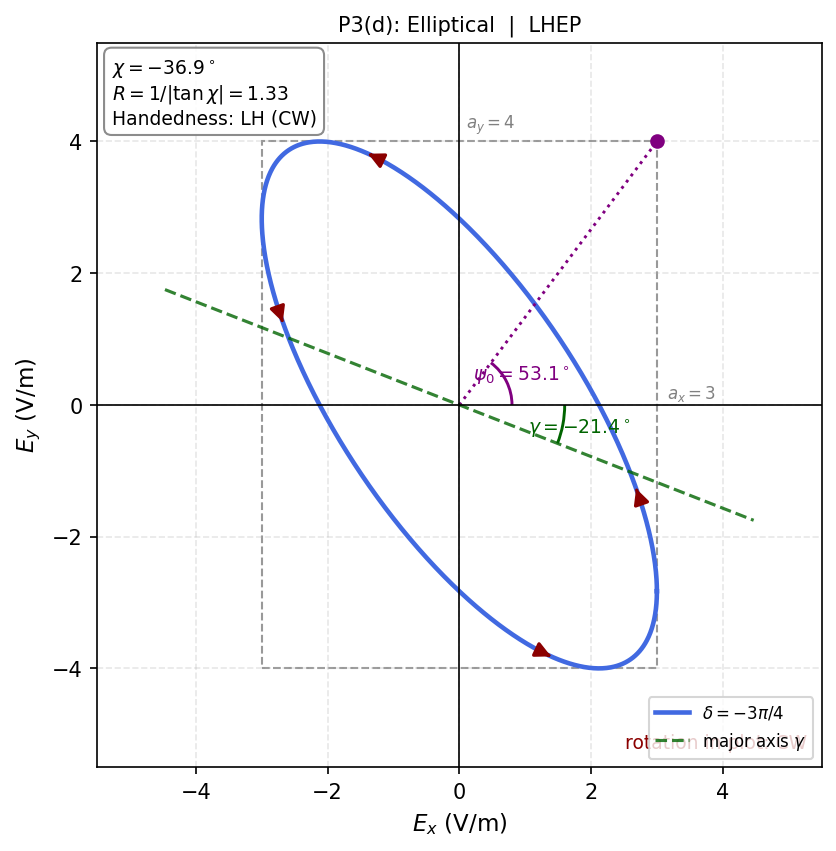
\includegraphics[width=0.55\linewidth]{HW2_P3d}\end{center}

\newpage
%======================================================
\probhead{4 --- Linear = RHC + LHC Decomposition}{8 pts}

\textbf{Setup:} Show $\tilde{\mathbf{E}} = a_x e^{-jkz}\hat{x}$ can be written as $\tilde{\mathbf{E}}_R + \tilde{\mathbf{E}}_L$.

\begin{cssnip}
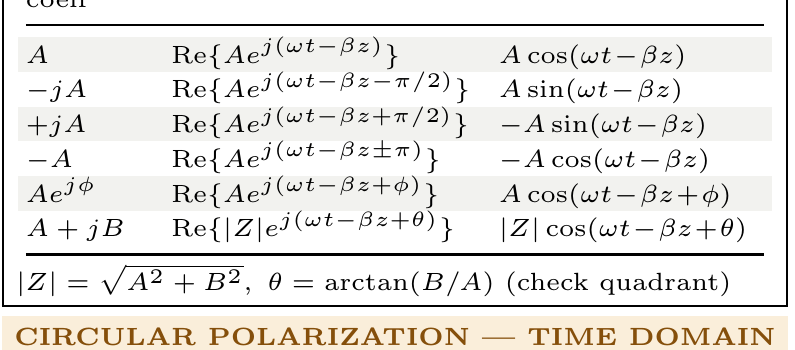
\includegraphics[width=0.98\linewidth]{cs_circular}
\end{cssnip}

\textbf{From the cheat sheet definitions:}
\[\tilde{\mathbf{E}}_R = a_R(\hat{x}-j\hat{y})e^{-jkz},\qquad
  \tilde{\mathbf{E}}_L = a_L(\hat{x}+j\hat{y})e^{-jkz}\]

\textbf{Try $a_R = a_L = a_x/2$:}
\begin{align*}
\tilde{\mathbf{E}}_R + \tilde{\mathbf{E}}_L
&= \big[(a_R+a_L)\hat{x} + j(-a_R+a_L)\hat{y}\big]e^{-jkz}\\
&= \big[a_x\,\hat{x} + j\cdot 0\cdot\hat{y}\big]e^{-jkz} = a_x e^{-jkz}\hat{x} = \tilde{\mathbf{E}}\;\checkmark
\end{align*}

\[\boxed{a_R = a_L = a_x/2}\]

%======================================================
\probhead{5 --- Dry Soil at 4 Frequencies (Loss Tangent Classification)}{24 pts}

\textbf{Setup:} $\varepsilon_r = 2.5$, $\mu_r = 1$, $\sigma = 10^{-4}$~S/m.

\begin{cssnip}
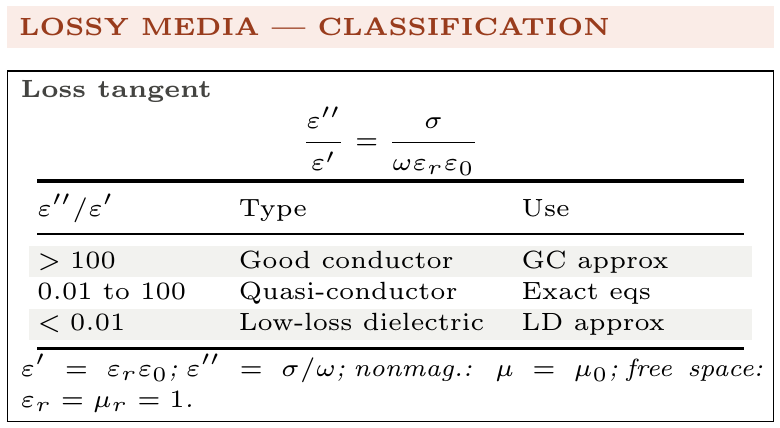
\includegraphics[width=0.49\linewidth]{cs_lossyclass}\hfill
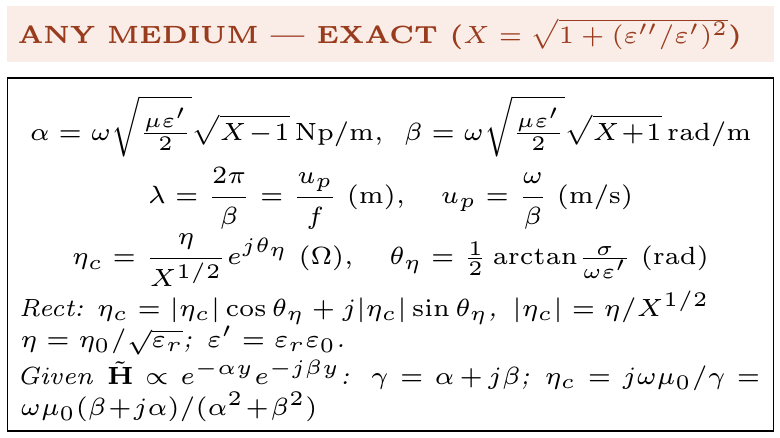
\includegraphics[width=0.49\linewidth]{cs_lossyexact}\\[4pt]
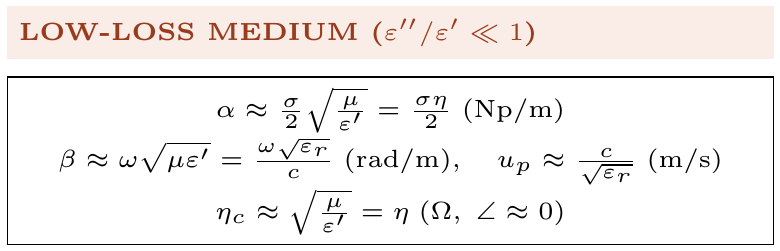
\includegraphics[width=0.49\linewidth]{cs_lowloss}\hfill
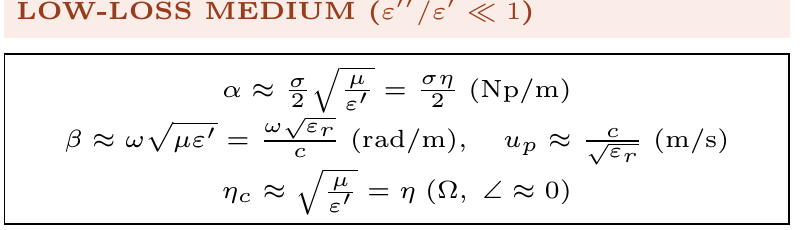
\includegraphics[width=0.49\linewidth]{cs_goodconductor}
\end{cssnip}

\textbf{Compute the loss tangent ratio:}
\[\frac{\varepsilon''}{\varepsilon'} = \frac{\sigma}{\omega\varepsilon_r\varepsilon_0} = \frac{\sigma/(2\pi\varepsilon_r\varepsilon_0)}{f} = \frac{7.193\times10^5~\text{Hz}}{f}\]

{\setlength{\tabcolsep}{8pt}
\begin{tabular}{cccc}
\toprule
$f$ & $\varepsilon''/\varepsilon'$ & Class & Use \\
\midrule
60 Hz & $1.20\times10^{4}$ & Good conductor & $\alpha\!\approx\!\beta\!\approx\!\sqrt{\pi f\mu\sigma}$ \\
1 kHz & $719.3$ & Good conductor & GC approx \\
1 MHz & $0.719$ & Quasi-conductor & Exact eqs \\
1 GHz & $7.19\!\times\!10^{-4}$ & Low-loss & LD approx \\
\bottomrule
\end{tabular}}

\textbf{(a) 60 Hz} (good conductor):
\[\alpha\approx\beta = \sqrt{\pi(60)(4\pi\!\times\!10^{-7})(10^{-4})} = 4.87\!\times\!10^{-6}~\text{Np/m, rad/m}\]
\[\lambda = 2\pi/\beta = 1.29\!\times\!10^{6}~\text{m},\quad u_p = \sqrt{4\pi f/\mu\sigma} = 7.74\!\times\!10^{7}~\text{m/s}\]
\[\eta_c \approx (1+j)\alpha/\sigma = (1+j)(0.0487)~\Omega\]

\textbf{(b) 1 kHz} (good conductor): same formulas, scale by $\sqrt{1000/60}\approx 4.08\times$:
\[\alpha\approx\beta = 1.99\!\times\!10^{-5}~\text{Np/m},\quad \lambda \approx 3.16\!\times\!10^{5}~\text{m}\]

\textbf{(c) 1 MHz} (quasi-conductor): use exact $X=\sqrt{1+(\varepsilon''/\varepsilon')^2}=\sqrt{1+0.719^2}=1.231$:
\[\alpha = \omega\sqrt{\tfrac{\mu\varepsilon'}{2}}\sqrt{X-1}~\text{Np/m},\quad
  \beta = \omega\sqrt{\tfrac{\mu\varepsilon'}{2}}\sqrt{X+1}~\text{rad/m}\]
\[\eta_c = \tfrac{\eta}{\sqrt{X}}e^{j\theta_\eta},\quad \theta_\eta = \tfrac{1}{2}\arctan(0.719)=17.7^\circ\]

\textbf{(d) 1 GHz} (low-loss dielectric):
\[\alpha\approx\tfrac{\sigma}{2}\sqrt{\mu/\varepsilon'} = \tfrac{10^{-4}}{2}\cdot\tfrac{377}{\sqrt{2.5}} = 0.0119~\text{Np/m}\]
\[\beta\approx\omega\sqrt{\mu\varepsilon'} = \tfrac{2\pi\!\times\!10^9\sqrt{2.5}}{3\!\times\!10^8} = 33.1~\text{rad/m}\]
\[\lambda \approx 2\pi/\beta = 0.190~\text{m},\;u_p\approx c/\sqrt{\varepsilon_r}=1.90\!\times\!10^{8}~\text{m/s},\;\eta_c\approx 238.4~\Omega\]

\newpage
%======================================================
\probhead{6 --- Phasor $\to$ Time Domain (Lossy)}{10 pts}

\textbf{Setup:} 300 MHz, nonmagnetic lossy, $\tilde{\mathbf{H}} = (\hat{x}-j4\hat{z})e^{-2y}e^{-j9y}$ A/m.

\begin{cssnip}

\includegraphics[width=0.49\linewidth]{cs_phasor}\hfill

\includegraphics[width=0.49\linewidth]{cs_kxE}
\end{cssnip}

\textbf{Read off:} $\omega = 6\pi\!\times\!10^8$ rad/s, $\alpha = 2$ Np/m, $\beta = 9$ rad/m, $\hat{k} = \hat{y}$.

\textbf{Time-domain $\mathbf{H}$} using the phasor table ($-j \to \sin$):
\[\mathbf{H}(y,t) = \big[\cos(\omega t - 9y)\,\hat{x} \,-\, 4\cos(\omega t - 9y + \tfrac{\pi}{2})\,\hat{z}\big]e^{-2y}~\text{A/m}\]

\textbf{Find $\tilde{\mathbf{E}}$} using $\tilde{\mathbf{E}} = -\eta_c(\hat{k}\times\tilde{\mathbf{H}})$, but for lossy we need $\eta_c$ first. Compute loss tangent:
\[\varepsilon''/\varepsilon' = (\alpha\beta\cdot 2)/(\omega^2\mu\varepsilon')\quad\text{(implicit from $\alpha,\beta$)}\]
Or compute $\eta_c = j\omega\mu_0/\gamma$ with $\gamma = \alpha + j\beta = 2 + j9$:
\[\eta_c = \tfrac{j(6\pi\!\times\!10^8)(4\pi\!\times\!10^{-7})}{2+j9}
  = \tfrac{j(753.98)}{2+j9}
  = \tfrac{j753.98\,(2-j9)}{4+81}
  = \tfrac{6785.8 + j1507.9}{85}
  \approx 79.8 + j17.7~\Omega\]

\textbf{Then $\hat{y}\times\hat{x} = -\hat{z}$, $\hat{y}\times\hat{z} = \hat{x}$:}
\[\tilde{\mathbf{E}} = -\eta_c\big(\hat{y}\times(\hat{x} - j4\hat{z})\big)e^{-2y}e^{-j9y}
  = -\eta_c(-\hat{z} - j4\hat{x})e^{-2y}e^{-j9y}\]
\[\tilde{\mathbf{E}} = \eta_c(j4\hat{x} + \hat{z})e^{-2y}e^{-j9y}~\text{V/m}\]

\textbf{Time domain:}
\[\mathbf{E}(y,t) = |\eta_c|\big[4\cos(\omega t-9y + \pi/2 + \theta_\eta)\,\hat{x} + \cos(\omega t-9y+\theta_\eta)\,\hat{z}\big]e^{-2y}\]
where $|\eta_c|\approx81.8$, $\theta_\eta = \arctan(17.7/79.8)\approx 12.5^\circ$.

%======================================================
\probhead{7 --- Direction of Travel and Poynting}{10 pts}

\textbf{Setup:} $\mathbf{E} = 3\cos(\pi\!\times\!10^7 t + kx)\hat{y} - 2\cos(\pi\!\times\!10^7 t + kx)\hat{z}$ V/m, nonmagnetic $\varepsilon_r=9$.

\begin{cssnip}

\includegraphics[width=0.49\linewidth]{cs_direction}\hfill
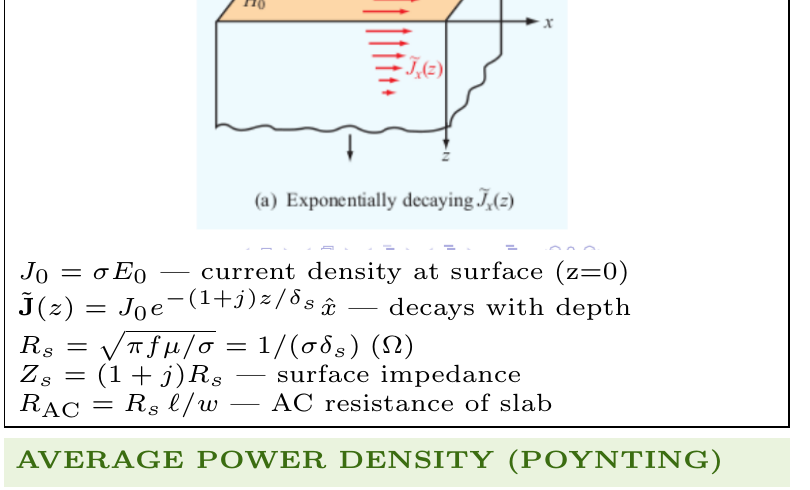
\includegraphics[width=0.49\linewidth]{cs_poynting}
\end{cssnip}

\textbf{Direction from the table:} argument is $\omega t + kx$ (plus sign $\Rightarrow$ wave travels in $-\hat{x}$).
\[\boxed{\hat{k} = -\hat{x}}\]
No $e^{-\alpha x}$ attenuation factor, so the medium is effectively lossless here.

\textbf{Intrinsic impedance:}
\[\eta = \eta_0/\sqrt{\varepsilon_r} = 377/3 \approx 125.7~\Omega = 40\pi~\Omega\]

\textbf{Poynting (lossless shortcut):} $|E_0|^2 = 3^2 + 2^2 = 13$.
\[\mathbf{S}_{\text{av}} = \tfrac{|E_0|^2}{2\eta}\hat{k} = \tfrac{13}{80\pi}(-\hat{x})~\text{W/m}^2 \approx -51.7~\text{mW/m}^2\,\hat{x}\]
\[\boxed{\mathbf{S}_{\text{av}} \approx -51.7~\text{mW/m}^2~\hat{x}}\]

\end{document}
